\newcommand{\ts}{\textsuperscript}

\newcommand{\fret}{f}


\newcommand{\veca}{\mathbf a}
\newcommand{\vecx}{\mathbf x}
\newcommand{\vecs}{\mathbf s}
\newcommand{\vecv}{\mathbf v}
\newcommand{\matV}{\mathbf V}
\newcommand{\vecz}{\mathbf z}
\newcommand{\vecX}{\mathbf X}
\newcommand{\mtrxsigma}{\mathbf{\Sigma}}
\newcommand{\argmax}[1]{\underset{#1}{\operatorname{argmax}}\;}
\newcommand{\argmin}[1]{\underset{#1}{\operatorname{argmin}}\;}


\newcommand{\colvec}[4]{ \begin{bmatrix} #1 \\ #2 \\ #3 \\ #4\end{bmatrix} }
\newcommand{\rowvec}[4]{ \begin{bmatrix} #1 & #2 & #3 & #4 \end{bmatrix} }



 % ---- Make typing equations easier -------------\c
\newcommand{\ahat}{\hat{\alpha}}
\newcommand{\C}{\boldsymbol{\zeta}}
\newcommand{\Like}{\mathcal{L}}
\newcommand{\Piz}{\boldsymbol\Pi_{Z}}
\newcommand{\Thetaparam}{\boldsymbol\Theta}
\newcommand{\HATThetaparam}{\hat{\boldsymbol\Theta}}
\newcommand{\thetaparam}{\boldsymbol\theta}
\newcommand{\thetahat}{\hat{\boldsymbol\theta}}
\newcommand{\limN}{\lim_{N\to\infty}}
\newcommand{\var}{\sigma^2}
\newcommand{\varhat}{\hat{\sigma}^2}
\newcommand{\z}{\mathbf{z}}
\newcommand{\ehat}{\hat{\mathbf{e}}}
\newcommand{\matZ}{\mathbf{Z}}
\newcommand{\matS}{\mathbf{S}}
\newcommand{\Z}{\mathbf{Z}}
\newcommand{\x}{\mathbf{x}}
\newcommand{\s}{\mathbf{s}}
\newcommand{\shat}{\mathbf{\hat{s}}}
\newcommand{\I}{\mathbf{I}}
\newcommand{\pz}{p(\mathbf{z})}
\newcommand{\pwz}{p(\omega|\mathbf{z})}
\newcommand{\Pwz}{P(\omega|\mathbf{z})}
\newcommand{\Pw}{P(\omega)}
\newcommand{\pwg}{p(\mathbf{w}|\gamma)}
\newcommand{\pwgk}{p(\mathbf{w}|\gamma_k)}
\newcommand{\Pzw}{P(\mathbf{z}|\omega)}
\newcommand{\w}{\omega}
\newcommand{\vecmu}{\text{\boldmath$\mu$}}
\newcommand{\what}{\hat\omega}
\newcommand{\Cost}{C(\hat\omega_i|\omega)}
\newcommand{\Risk}{R(\hat\omega_i|\z)}
\newcommand{\E}{\mathrm{E}} 
 % -----------------------------------------------

\newcommand{\vecr}{\mathbf r}
% section describing the guitar tuner harmonic summation
\newcommand{\NFFT}{\texttt{NFFT}}
\newcommand{\N}{\texttt{N}}
\newcommand{\dur}{\texttt{dur}}
\newcommand{\vecf}{\mathbf f}
\newcommand\numberthis{\addtocounter{equation}{1}\tag{\theequation}}
\newcommand{\HL}{\bm{HL}}
\newcommand{\PSNR}{\textit{PSNR}}
\newcommand{\SNR}{\textit{SNR}}
\newcommand{\PSNRvec}{\mathbf{PSNR}}
\newcommand{\SNRvec}{\mathbf{SNR}}
\newcommand{\RMSE}{\textit{RMSE}}
%% -----------------------------------------------------
\newcommand{\vectheta}{\text{\boldmath$\theta$}}
\newcommand{\vecphi}{\text{\boldmath$\phi$}}
\newcommand{\vecPhi}{\text{\boldmath$\Phi$}}
\newcommand{\vecalpha}{\text{\boldmath$\alpha$}}
\newcommand{\vecalphahat}{\text{\boldmath${\widehat\alpha}$}}

\newcommand{\norm}[1]{\left\lVert#1\right\rVert}

%
%\newcommand{\ts}{\textsuperscript}

%\newcommand{\veca}{\mathbf a}
% \newcommand{\vecX}{\mathbf X}
% \newcommand{\vecmu}{\mathbf{\mu}}
%\newcommand{\mtrxsigma}{\mathbf{\Sigma}}
% \newcommand{\argmax}[1]{\underset{#1}{\operatorname{arg}\,\operatorname{max}}\;}
% \newcommand{\argmin}[1]{\underset{#1}{\operatorname{arg}\,\operatorname{min}}\;}


% \newcommand{\colvec}[4]{ \begin{bmatrix} #1 \\ #2 \\ #3 \\ #4\end{bmatrix} }
% \newcommand{\rowvec}[4]{ \begin{bmatrix} #1 & #2 & #3 & #4 \end{bmatrix} }
 \newcommand{\symvec}[1]{{\mbox{\boldmath $#1$}}}
 \newcommand{\symmat}[1]{{\mbox{\boldmath $#1$}}}
\section{signal model}
The signal model is derived from the string vibrations, thus we start by describing the activation from the guitar pick. 
%
\begin{figure}[h!]\
  \centering
  \centerline{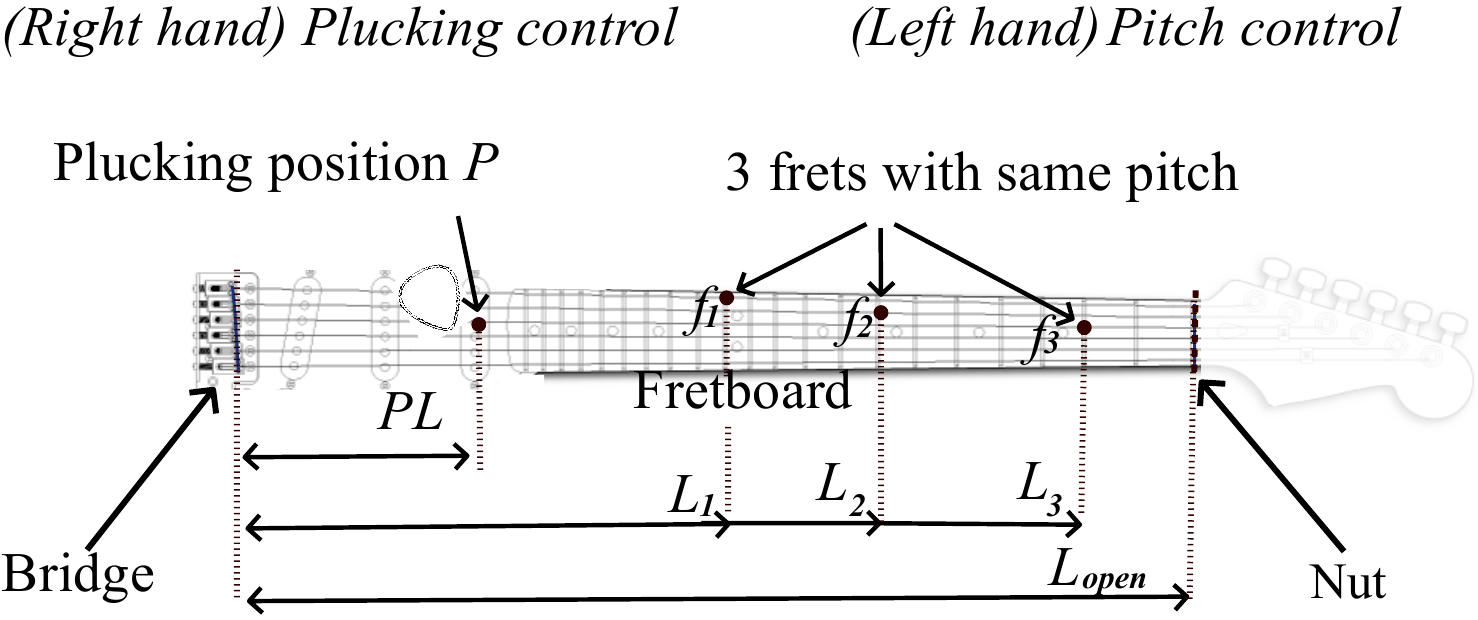
\includegraphics[width=1\columnwidth]{img/fender_drawing4.png}}
  \caption{The plucking position is controlled by the right hand while the left hand controls pitch using the fretboard. Similar pitch is produced in various positions. Source: Adapted from~\cite{phillips}.
  }\label{fig:guitar_overview}\vspace{-2mm}
\end{figure}
%
The string has an initial deflection $\delta$ at the plucking position, which is at the $P$th fraction of its length $(0<PL<L)$, where $L$ is the length of the vibrating string (see i.e.,~Fig.~\ref{fig:guitar_overview}). 
%The displacement $y$ defined by the 1D wave equation: %
%\begin{equation}
% $\frac{\partial^2y}{\partial t^2} = c^2\frac{\partial^2y}{\partial l^2}$,
%\end{equation}
%
%where $c$ is the transverse wave speed. 
Assuming that the string is not ideal and is pinned at locations $l=0$ and $l=L$, its general solution can be written as~\cite{fletcher:physics_of_musical_instruments}
%
\begin{equation}\label{eq:modalSum}
    y(l,t) = \sum_m C_m\sin(\psi_mt+\phi_m)\sin\kappa_ml,
\end{equation}
%
with the amplitude $C_m$ and wave number $\kappa_m = \omega_m / c$ of the $m$th mode where $m\in \mathbb{Z}^+$. The instantaneous frequencies $\psi_m$ follow the piano model proposed in~\cite{fletcher:piano_model} as 
\begin{equation}\label{eq:pianoModel}
  \psi_m(\omega_0,B) = m \omega_0 \sqrt{1+B m^2} \quad [\text{s}^{-1}], 
\end{equation}
with fundamental frequency $\omega_0$ and inharmonicity coefficient $B$ to be discussed shortly. 

Assuming the initial displacement to be triangular and no initial velocity $\frac{\partial y}{\partial t} = 0 \, \forall\, l$, the $m$th amplitude $C_m$ is defined by the Fourier sine series as~\cite{donkin:acoustics,fletcher:principles_of_vibration_and_sound}
\begin{equation}
    C_m = \frac{2\delta}{m^2\pi^2P(1-P)}\sin(m\pi P), \quad [\cdot].
\end{equation}
It can be observed that the spectral envelope is sinusoidal along the partials, and dependent only on the plucking position $P$ scaled by $m^{-2}$ for the $m$th mode.

On the guitar we assume that a pickup is measuring the displacement $y(l,t)$ in close proximity to the string at location $l\!=\!\lambda$. At the discrete time instance $n$ the observed signal $x(n)$ is uniformly sampled such that is proportional to $y$, i.e.,
\begin{equation}
     x(n)  \vert_{l=\lambda} \propto y(\lambda, t).
\end{equation}   
We parametrize $x(n)$ as proposed in~\cite{hjerrild::icassp19}, where $x(n)$ is modeled as an inharmonic sinusoidal part and a noise part, i.e.,  
\begin{equation}\label{eq:sigmod1}
  x(n)\! =  \!\sum\limits_{m=1}^{M}\!\! \alpha_{m} \exp\big({j\psi_m(\omega_0,B) n}\big)+v(n),
\end{equation}
where $\omega_0$ is the fundamental frequency, $\alpha_{m}$ is the complex amplitude of the $m$th partial, $M$ is the number of partials, $v(n)$ is noise and $\psi_m(\omega_0,B)$ is defined in~\eqref{eq:pianoModel}.
%
 At time instance $n$, the observed signal vector $\vecx \in \mathbb{C}^N$ is represented as $\vecx = [x(0) \, x(1) \, \cdots \, x(N-1)]^T$, with $T$ denoting the transpose. %Do we need this?
%A complex signal can ease both notation and computational complexity and a real-valued signal is converted to complex by using the Hilbert transform~\cite{LawrenceMarple1999}. 
 %To ease on notation we leave out the $(\omega_0, B)$ in the following, and define a sinusoidal matrix $\matZ =& \left[ \vecz(\psi_1) \: \vecz(\psi_2) \: \cdots \: \vecz(\psi_M)\right] \matZ \in \mathbb{C}^{N\times M}$, where each column is $\vecz(\psi_m) =& \left[ 1 \: e^{j\psi_m} \: e^{j\psi_m2} \: \cdots \: e^{j\psi_m(N-1)} \right]^{T}$ 
In matrix notation the observed signal is% modeled as
\begin{equation}\label{eq:xZa}
  \vecx = \matZ \vecalpha + \vecv,
\end{equation} 
where $\vecalpha\!=\! [\alpha_1 \: \cdots \: \alpha_M]^T$ is a vector containing complex amplitudes, $\vecv\! =\! [v(0) \: v(1) \: v(N-1)]^T$ contains all noise terms and the Vandermonde matrix $\matZ\! \in\! \mathbb{C}^{N\times M}$ contains all inharmonic sinusoids as specified in~\cite{hjerrild::icassp19}.
%%\begin{align}
%$  \matZ =& \left[ \vecz(\psi_1) \: \vecz(\psi_2) \: \cdots \: \vecz(\psi_M)\right], $ and
%$ \vecz(\psi_m) =& \left[ 1 \: e^{j\psi_m} \: e^{j\psi_m2} \: \cdots \: e^{j\psi_m(N-1)} \right]^{T},$
%%\end{align}
We denote the unknown and deterministic parameters that comprises the feature set with $\vectheta$, i.e.
\begin{equation}\label{eq:theta_parameters}
  \vectheta = \{\omega_0, B, \vecalpha\}.
\end{equation}
The amplitudes $\vecalpha$ are linear, while the fundamental frequency $\omega_0$ and inharmonicity $B$ both are non-linear. 
The amplitude estimates $\vecalphahat$ has been shown to be sufficient for estimating the plucking position $\widehat{P}$ in the fretted string scenario~\cite{hjerrild::icassp19}, while $\{\widehat\omega_0, \widehat B \} $ was sufficient for classification of string and fret in~\cite{barbancho:inharmonicity_tablature,michelson2018_aes}.